\chapter{Collision Data Samples}
\label{chap:data}
\section{Data Periods and Good Run List}
\label{EventSel:GRL}

\indent This analysis uses the LHC proton-proton collision data at a centre-of-mass energy of $\sqrt{s}$=13 TeV that was collected by ATLAS in 2015 and 2016. \\

\indent We select data where all relevant subdetector parts are running without defects and the quality of data is good.  This is done by requiring the data pass a good run list (GRL).  The good run list is compiled from data that pass manual and automated checks on both detector hardware and the kinematics of reconstructed physics objects.  \\

\indent The GRLs used for the 2015 dataset is {\tt data15\_13TeV.periodAllYear\_DetStatus-v79-repro20-02\_DQDefects-00-02-02\_PHYS\_StandardGRL\_All\_Good\_25ns.xml}.  \\
\indent The GRL for the 2016 data is {\tt data16\_13TeV.periodAllYear\_DetStatus-v83-pro20-15\_DQDefects-00-02-04\_PHYS\_StandardGRL\_All\_Good\_25ns.xml}.

\indent The dataset after GRL selection corresponds to a total integrated luminosity of $\intlumi \pm 1.15$ $\ifb$.  The total integrated luminosity as a function of time for 2015 and 2016 before the requirement of an GRL is shown in Figure \ref{fig:data2015-2016}.\\

\begin{figure}[h!]
  \begin{center}
    \begin{subfigure}[b]{0.40\textwidth}
        \includegraphics[width=\textwidth]{figures/Data/IntLumi2015.png}
                \caption{ }
    \end{subfigure}
    \begin{subfigure}[b]{0.40\textwidth}
        \includegraphics[width=\textwidth]{figures/Data/IntLumi2016.png}
                \caption{ }
    \end{subfigure}
\end{center}
\caption{Distribution of the amount of data delivered by the LHC and recorded by ATLAS vs time in 2015 (a) and 2016 (b) }
\label{fig:data2015-2016} 
\end{figure}

\indent Peak luminosity reached $1.38 \times 10^{34}$  cm$^{-2}$ sec$^{-1}$ in 2016.  Taking data at this high rate means we expect multiple p-p interactions in every bunch crossing.  The average number of interactions per bunch crossing, $\braket{\mu}$, is 13.7 in 2015 and 23.2 in 2016.  The distribution of the mean number of interactions per bunch crossing is given in Figure \ref{fig:nVtx}.   \\

\begin{figure}[h!]
  \begin{center}
    \includegraphics[width=0.75\textwidth]{figures/Data/mu_2015_2016_LHCC.png}
\end{center}
\caption[Distribution of the mean number of interactions per bunch crossing weighted by integrated luminosity for 2015 and 2016 ATLAS data taking. ]{ Distribution of the mean number of p-p interactions per bunch crossing weighted by integrated luminosity for 2015 and 2016 ATLAS data taking.  The on average 22.9 p-p interactions occur in every bunch crossing in the 2015+2016 ATLAS dataset. }
\label{fig:nVtx} 
\end{figure}

\indent In order to keep data flow to a manageable size, ATLAS only records events if a trigger is fired.  The ATLAS trigger system is summarized in chapter \ref{chap:trigger}.  This analysis uses the lowest unprescaled $\met$ trigger for each data taking period.  This trigger threshold was set at 70 $\gev$ to 110 $\gev$ depending on the data taking period. The trigger efficiency curve as a function of offline $\met$ for select $\met$ triggers can be seen in Figure \ref{fig:trigTurnON}. \\

\chapter{Event Preselection}
\label{chap:Selection_EventPreselection}

\indent We require that the event pass a few basic selections designed to reject non-collision backgrounds and events with large amounts of calorimeter noise.  Together these basic selections are referred to as event cleaning and jet cleaning.  \\ %These basic selections are applied to all regions.  

\indent A brief description of the preselection requirements is given below: Details on all object definitions can be found in chapter \ref{chap:objects}. \\

\begin{description}
\item[Cut 1] Data events must satisfy the Good Runs List (GRL) requirement described in chapter \ref{EventSel:GRL}.  This ensures all relevant subdetectors of ATLAS are operating normally during data taking. 
\item[Cut 2] Remove events with noise bursts and possible incomplete events due to the TTC reset procedure from the data. Data events must have no errors flagged in the calorimeter and ID.  The following error flags must be zero: larError $== 0$, tileError $== 0$, SCT error $==0$, and coreFlags $\&0x4000 == 0$.
\item[Cut 4] Require that at least one reconstructed primary vertex exists.
\item[Cut 5] Events must not contain any {\tt BadLoose} jets with $\pT > 20 \gev$ (at any \eta\ range). Bad quality jets indicate the presence of calorimeter noise or non-collision backgrounds. Both can lead to poor $\met$ reconstruction. Hence, the whole event is rejected.  {\tt BadLoose} jets are defined in jet quality selection in section \ref{sec:jet:quality}.  
\item[Cut 6] The event must not contain any cosmic muons.  Cosmic muons are identified as muons with large impact parameters  ($|z_0| > 1$ mm and $|d_0| > 0.2$ mm).  Only {\tt Baseline} muons after overlap removal are considered in cosmic muon identification.
\item[Cut 7] The event must not contain any {\tt Baseline} muons with $|\sigma(q/p)/|(q/p)| > 0.2$.  Muons with large fractional uncertainty often result from kaon decays or poorly reconstructed inner detector tracks that are incorrectly matched to muon spectrometer segments. These muons may result in misreconstructed $\met$ so the whole event is rejected.
\end{description}

%\indent On top of these basic requirements, additional preselection requirement are applied to each control region, VR and signal region depending on the number of leptons required in the respective region.  \\

\section{zero-lepton Preselection}

\indent All zero-lepton regions require the following set of preselections given in Table \ref{tab:0Lcommon}.  We require exactly zero {\tt Baseline} leptons to vote events containing electrons and muons.  \\

\indent All zero-lepton regions trigger on $\met$ using the lowest unprescaled $\met$ trigger for that data period.  An offline selection of $\met > 250 \gev$ is required to ensure that all accepted events are on the trigger efficiency plateau.  The trigger efficiency curve as a function of offline $\met$ for select $\met$ triggers can be seen in Figure \ref{fig:trigTurnON}. \\

\begin{table}[h!]
  \caption{ The zero-lepton preselection criteria common to all zero-lepton regions.}
  \label{tab:0Lcommon}
  \begin{center}
  \setlength{\tabcolsep}{0.0pc}
    \begin{tabular}{lc} \hline\hline
      \multicolumn{2}{c}{GRL, Event Cleaning and Jet Cleaning} \\ \hline
      \multicolumn{2}{c}{$\met$ Trigger}   \\ \hline
      $\met$ & $> 250\GeV$ \\ 
      $N_{\rm{{\tt Baseline}~lep}}$ & 0 \\ 
      \antikt\ $R=0.4$ {\tt Signal} jets & $\ge 4,~\pt>80,80,40,40 \gev$ \\ 
      $b$-tagged {\tt Signal} jets & $\ge1$ \\ 
      % $\dphijettwomet$ & $> \pi/5$ \\ 
        & \\ [-2.5ex] 
      $\dphijettwomet$ & $> 0.4$ \\ 
              & \\ [-2.5ex] 
      $\mettrk$  & $> 30 \gev$ \\ 
       & \\ [-2.5ex]
      $\dphimettrk$ & $<\pi/3$ \\  \hline
      % & \\ [-2.5ex] \hline
      % $\tau$ veto & yes \\ \hline
      % $\mtbmetmindphi$ & $> 175 \gev$ \\ \hline \hline
    \end{tabular}
  \end{center}
\end{table}

\indent We also require at least four {\tt Signal} jets with a minimum $\pt$ of $(80,80,40,40) \gev$ in the event.  At least one {\tt Signal} jet must be b-tagged at the 77\% working point.  These jet energy and multiplicity requirements are loose and will be superseded by more stringent selections. \\

%Any zero-lepton region requires the selections given in Table \ref{tab:0Lcommon}. \\

\indent We also include a number of selections aimed specifically at rejecting QCD multijet background.  The primary reason that QCD multijet background can pass the $\met > 250 \gev$ requirement is due to misreconstructed jets.  QCD multijet processes produce little intrinsic $\met$ but multijet background can have large reconstructed $\met$ if any of the energetic jets are mismeasured.  For example, an extremely energetic jet may punch through the calorimeter and deposit part of its energy outside the calorimeter.  This lost $E_T$ may be reconstructed as $\met$.  \\

\indent The $\dphijettwomet > 0.4$ requirement ensures that the $\met$ is not collinear with either of the two most energetic jets in the event.  $\dphijettwomet$ is defined in equation \ref{eqn:dphijetmet}. \\

\begin{equation}
\dphijettwomet = \min_{2~highest~pt~jets} |\Delta \phi ( jet, \met ) |
\label{eqn:dphijetmet}
\end{equation}

\indent This provides strong rejection against fake $\met$ resulting from a single misreconstructed energetic jet.  \\

\indent In addition, we require a loose agreement between two methods of reconstructing missing transverse energy, $\met$ and $\mettrk$.  $\mettrk$, defined in equation \ref{eqn:mettrkReco}, is reconstructed using a negative vector sum of all accepted ID tracks.  Track $\met$ is very robust against pile-up conditions as ID tracks can be matched to a primary vertex but $\mettrk$ neglects the presence of neutral particles.  We found that a loose requirement of $\mettrk > 30 \gev$ and a loose agreement between $\met$ and $\mettrk$ in $\phi$ form an efficient discriminant against QCD multijet background. \\

\indent  Distributions of select kinematic variables after the zero-lepton preselection can be seen in Figure \ref{fig:presel:dist}.  The signal and background have similar $\met$ distributions.  This demonstrates that $\met$ variable provides little separation power between the signal and background. \\  

\begin{figure}[h!]
  \begin{center}
      \begin{subfigure}[b]{0.40\textwidth}    
    	 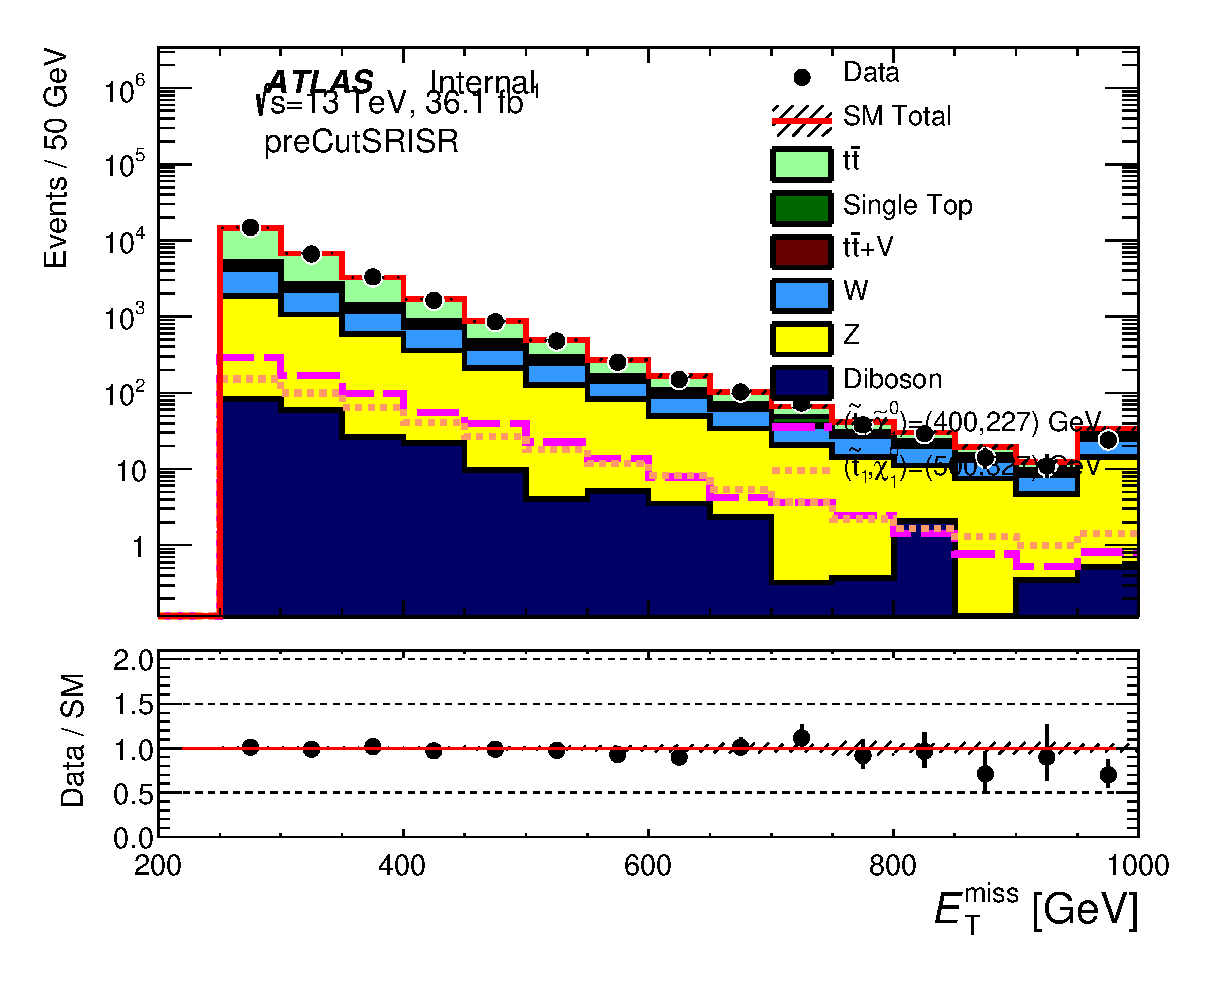
\includegraphics[width=\textwidth]{figures/plotRegion/Met_preCutSRISR_log.eps}
                \caption{ }
    \end{subfigure}
        \begin{subfigure}[b]{0.40\textwidth}    
    	 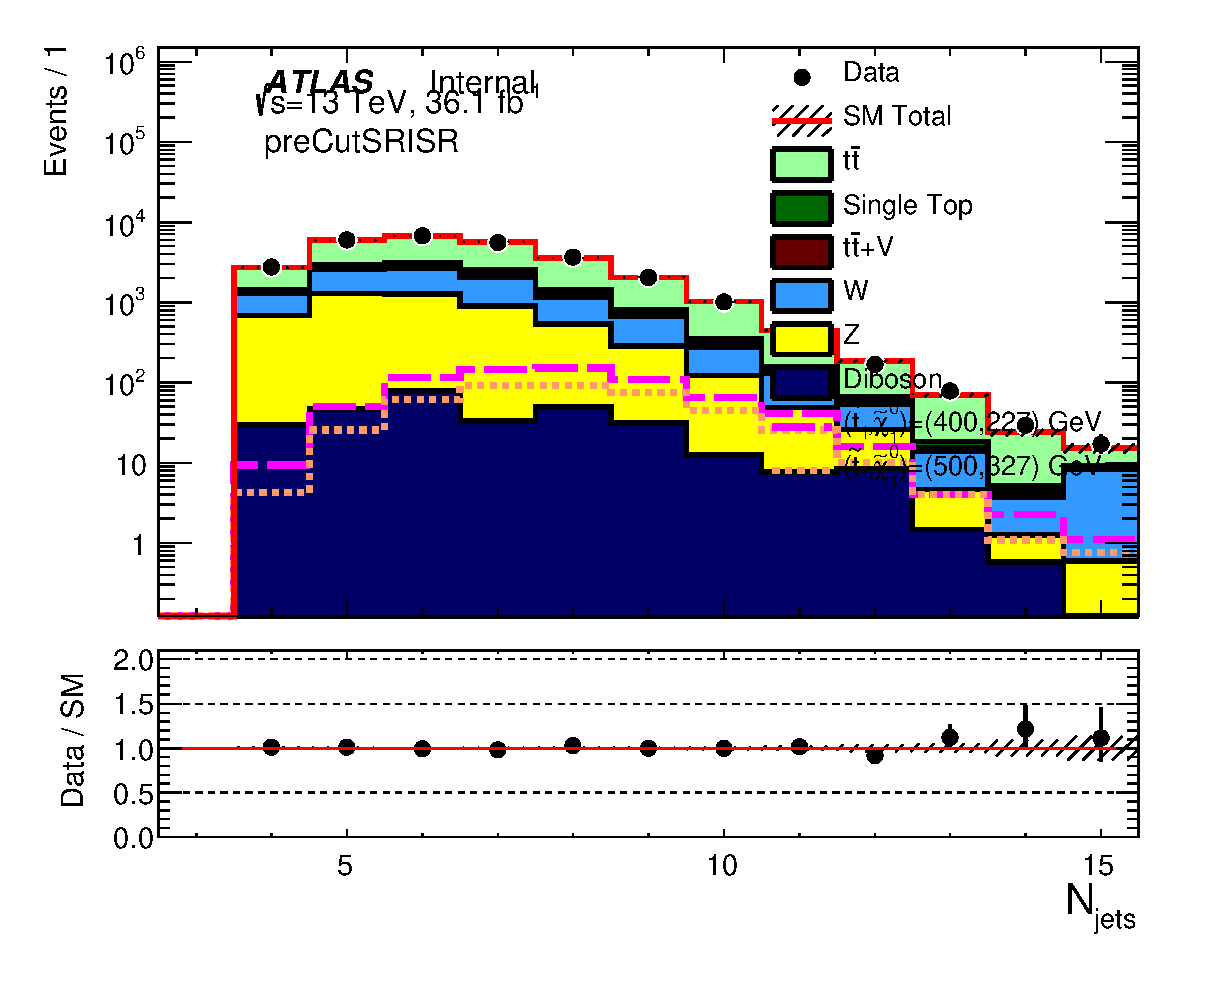
\includegraphics[width=\textwidth]{figures/plotRegion/NJets_preCutSRISR_log.eps}
                \caption{ }
    \end{subfigure}
    \begin{subfigure}[b]{0.40\textwidth}    
    	 \includegraphics[width=\textwidth]{figures/plotRegion/Ht_preCutSRISR_log.eps}
                \caption{ }
    \end{subfigure}
    \begin{subfigure}[b]{0.40\textwidth}    
    	 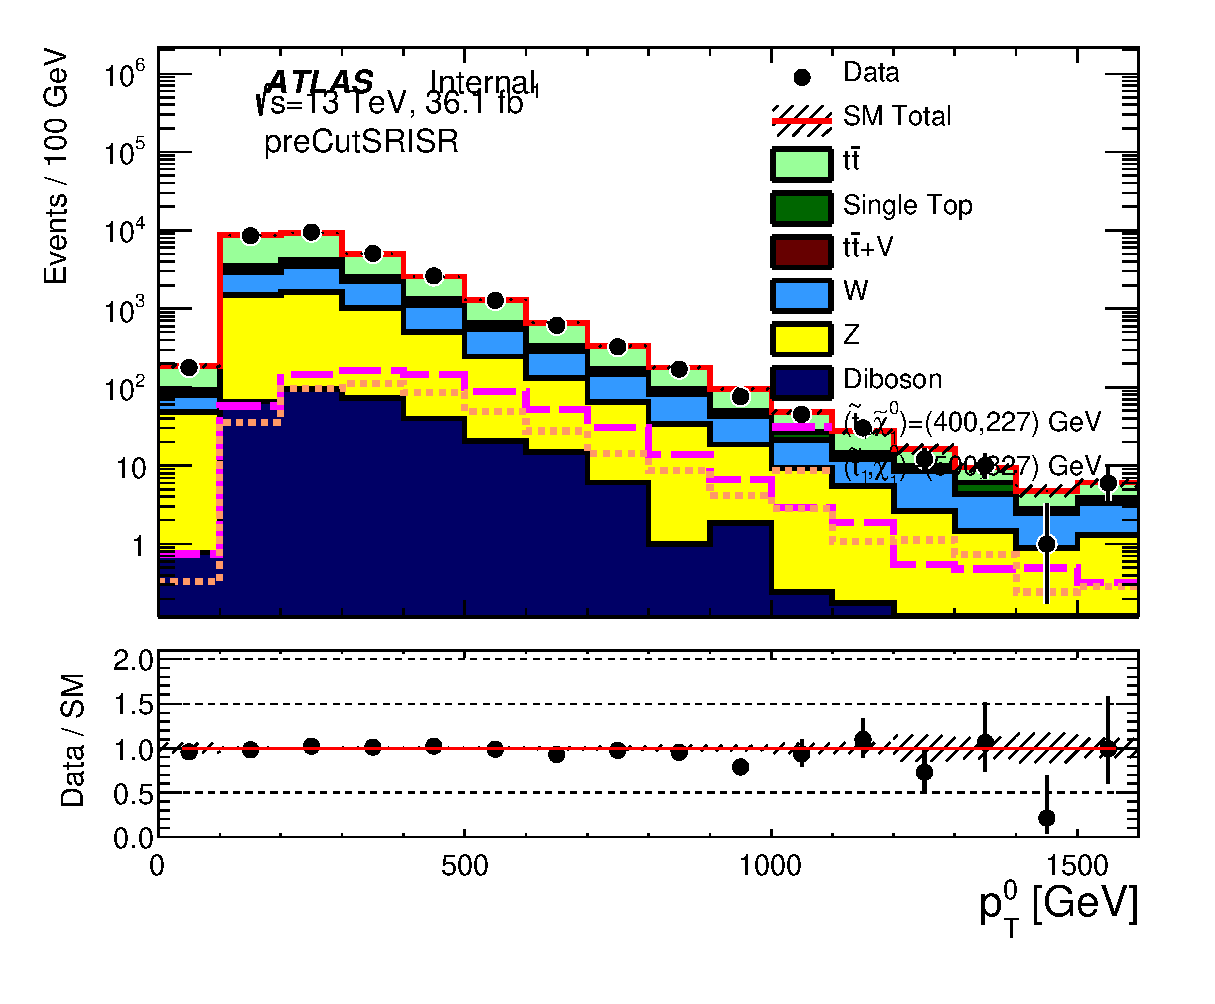
\includegraphics[width=\textwidth]{figures/plotRegion/JetPt_0__preCutSRISR_log.eps}
                \caption{ }
    \end{subfigure}
    \begin{subfigure}[b]{0.40\textwidth}    
    	 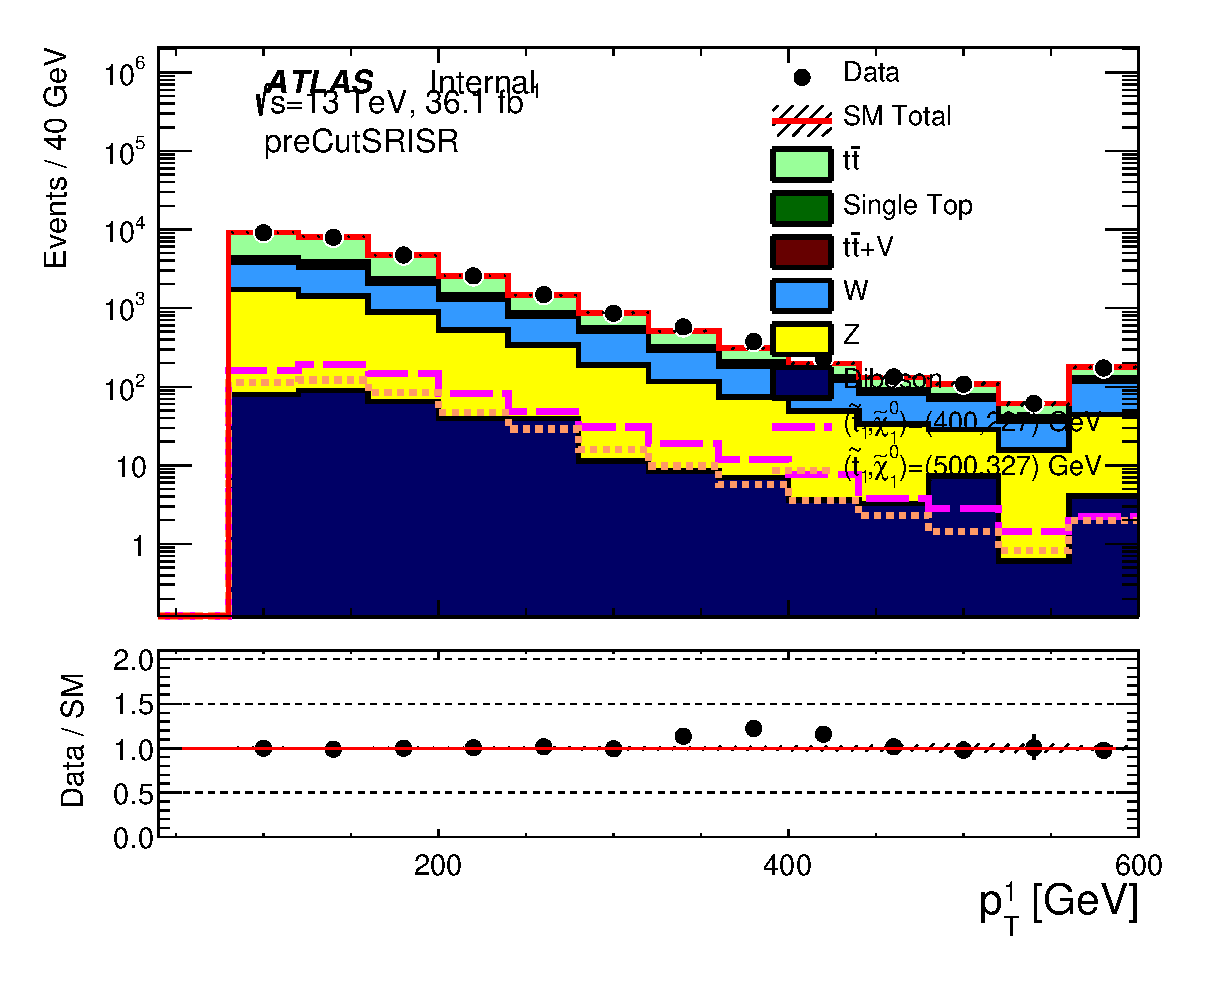
\includegraphics[width=\textwidth]{figures/plotRegion/JetPt_1__preCutSRISR_log.eps}
                \caption{ }
    \end{subfigure}
    \begin{subfigure}[b]{0.40\textwidth}    
    	 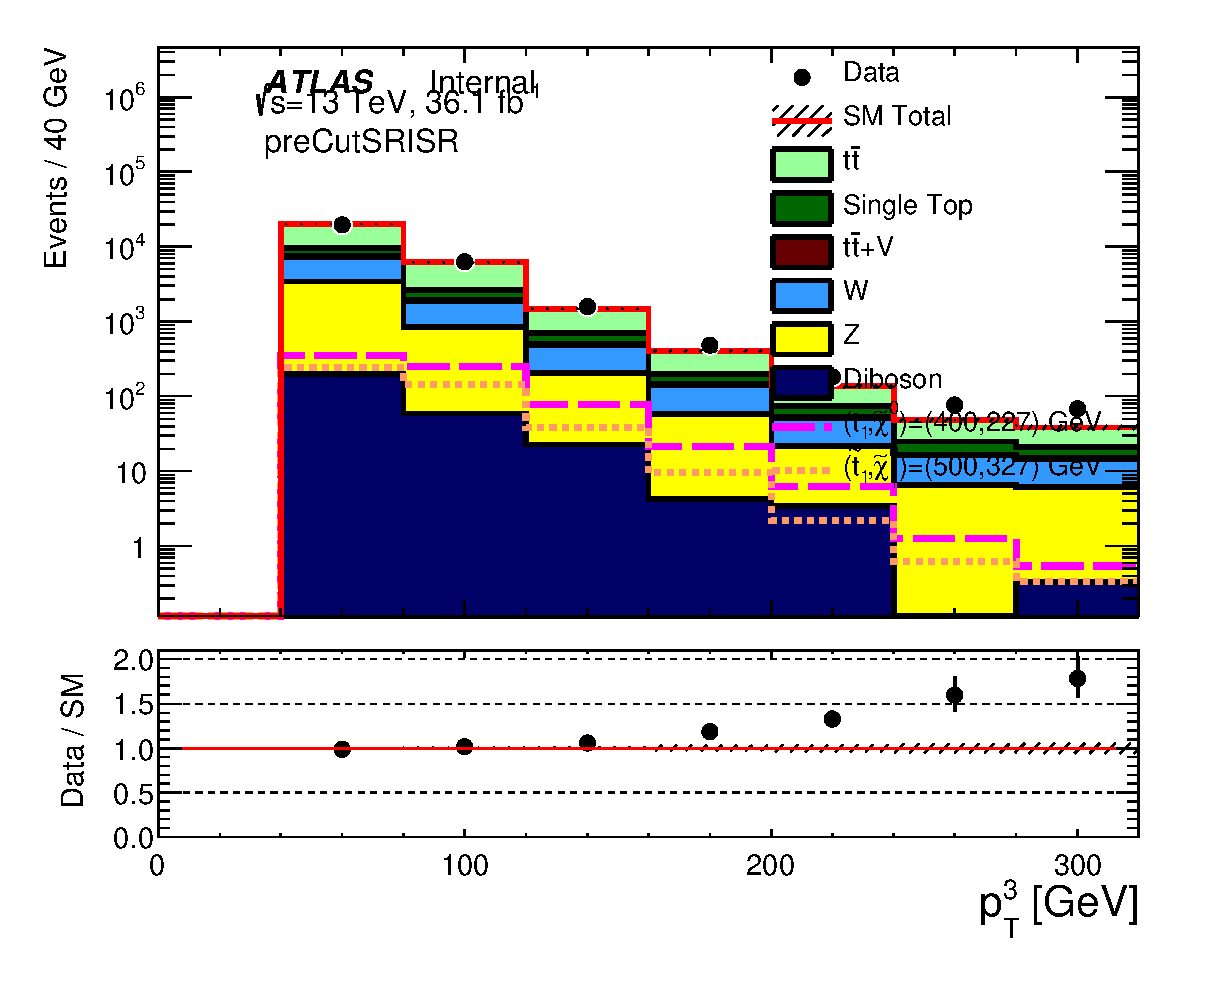
\includegraphics[width=\textwidth]{figures/plotRegion/JetPt_3__preCutSRISR_log.eps}
               \caption{ }
    \end{subfigure}
     \caption[Kinematic variable distributions after the zero-lepton preselection.]{ Kinematic variable distributions after the zero-lepton preselection; (a) $\met$ (b) number of jets (c) $\HT$ (d) $\pt$ of the highest $\pt$ jet (e) $\pt$ of the 2nd highest $\pt$ jet (f) $\pt$ of the 4th highest $\pt$ jet. SM backgrounds are displayed as the solid stacked histograms.  Stop signals with $(m_{\stop}, m_{\ninoone}) = (400 \gev,227 \gev)$ and $(500 \gev, 327 \gev)$ are shown as dashed histograms.  The data/MC ratio is shown in the lower panel. }
  \label{fig:presel:dist}
    \end{center}
\end{figure}

\section{One-Lepton Preselection}

\indent We use one-lepton regions as control regions to estimate the background in the zero-lepton signal region.  The MC is normalized to data in the control region through a combined fit to all control regions. This normalization is also applied to the background MC in the signal region.  In this way, we directly measure the amount of background in the control region using data and only rely on simulation to extrapolate between the control region and the signal region.  As such, the one-lepton control regions are designed to be kinematically similar to the zero-lepton signal region.  This minimizes the extrapolation between the two regions and minimizes the uncertainty on the expected background rates in the signal region. \\

\indent For this reason, the preselection for one-lepton regions is similar to the zero-lepton preselection.  Both zero and one-lepton regions trigger using the $\met$ triggers defined in chapter \ref{chap:trigger}.  We also require $\met > 250 \gev$ to ensure that we are on the trigger efficiency plateau.  \\

\indent The one-lepton selections use {\tt Signal} leptons instead of the {\tt Baseline} leptons used in zero-lepton regions.  The one-lepton regions use lepton momentum information and therefore require higher quality leptons. \\

\indent The one-lepton preselection is summarized in Table \ref{tab:1Lcommon}. \\

\begin{table}[h!]
  \caption{ The one-lepton preselection criteria common to all one-lepton regions.}
  \label{tab:1Lcommon}
  \setlength{\tabcolsep}{0.0pc}
  \begin{center}
    \begin{tabular}{lc} \hline\hline
      \multicolumn{2}{c}{GRL, Event Cleaning and Jet Cleaning} \\ \hline
      \multicolumn{2}{c}{$\met$ Trigger} \\ \hline
      $\met$ & $> 250\GeV$ \\ 
      $N_{\rm{{\tt Signal}~lep}}$ & 1 \\
    $N_{jets}$ & $\ge 4$ \\ 
      $b$-tagged {\tt Signal} jets & $\ge1$ \\ 
                   & \\ [-2.5ex] 
      $\dphijettwomet$ & $> 0.4$ \\
             & \\ [-2.5ex] \hline
    \end{tabular}
  \end{center}
\end{table}

\indent The lepton veto rejects single electron and single muon $\ttbar$ decays and the all hadronic $\ttbar$ decay produces little $\met$.  For this reason, the biggest background in the signal region comes from SM $\ttbar$ where one top decays via the hadronic tau channel and the other top decays via the hadronic channel.  The $W$ from $W$+jets and single-top backgrounds in the signal region also decays predominantly through the hadronic tau channel.  For this reason, the majority of SM backgrounds in the signal region contains a hadronic tau.  \\

\indent We expect many parallels between the electron and muon decay channels and the tau decay channel because of lepton universality.  Therefore, we use the electron or muon in the one-lepton channel to mimic the hadronic tau in the signal region.  Since we do not distinguish between hadronic tau jets and other jets in the signal region, both {\tt Signal} leptons and {\tt Signal} jets are counted as ``jets'' in one-lepton regions. \\

\indent The $\mettrk > 30 \gev$ and $\dphimettrk < \pi/3$ requirements are removed because the QCD multijet contribution to one-lepton regions is negligible.  The $\dphijettwomet > 0.4$ selection is kept because it provides a closer modeling of the phase space in the signal region. \\


